\chapter{Análisis}
\lhead{Análisis}

\begin{cabstract}
En el que se describen los diferentes aspectos de la fase de análisis del sistema desde una perspectiva holística.
\end{cabstract}

Recoger todos los aspectos de análisis de un sistema como el creado en un único capítulo es contraproducente para la adecuada comprensión de los diferentes procesos llevados a cabo. Es por ello que en el presente capítulo se detallarán los diferentes aspectos de análisis llevados a cabo para el sistema como unidad, que ayudarán a la identificación de las necesidades a satisfacer por el mismo. Dichos aspectos serán de utilidad durante el desarrollo de las restantes etapas de análisis centradas en cada uno de los diferentes componentes del sistema.

\section{Identificación de componentes}

Todo sistema se compone del conjunto de integrantes y las relaciones que estos mantienen entre ellos mismos y su entorno, con una serie de objetivos a cumplir a través de dichas interacciones. El límite entre el sistema y su entorno es de necesario estudio para comprender los diferentes procesos de  entrada y salida que se desarrollan.

\subsection{Componentes principales} 

Los componente principales del sistema son los nodos Raspberry Pi, que serán los encargados de la ejecución de las diferentes tareas solicitadas por los usuarios del sistema.

\subsection{Componentes secundarios}

En una primera instancia del proceso de análisis no se detalla ningún tipo de nodo secundario, delegando en los componentes principales del sistema todas las tareas a llevar a cabo.

Sin embargo, en las diferentes etapas de desarrollo se plantea el uso de varios componentes secundarios para la gestión de una serie de tareas cuya ejecución en el conjunto de componentes principales es dificultosa, o su delegación beneficia al conjunto de nodos principales. En cualquier caso, dichas tareas pueden ser asignadas a los componentes principales en cualquier momento (ver \ref{chapter:serviciosauxiliares}).

\begin{figure}[H]
	\centering
	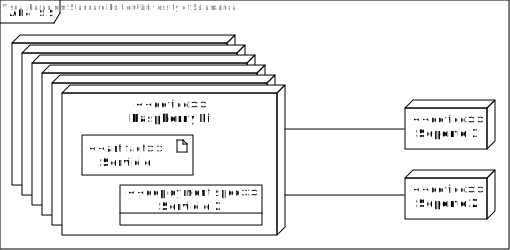
\includegraphics[width=0.8\textwidth]{Chapter4/Figures/Análisis-Componentes}
	\caption[Análisis de componentes]{Análisis de componentes del sistema}
	\label{analisis:componentes}
\end{figure}

\subsection{Interconexión}

Se plantea el uso de cableado físico Ethernet para la comunicación entre los diferentes nodos. Este tipo de conexión es soportada por todos los componentes anteriormente mencionados, y se cuenta con dicho cableado en la infraestructura del centro (ver \ref{dominioproblema:infraestructura}).

\section{Información gestionada por el sistema}

Se plantea un conjunto de requisitos de información gestionados por el sistema pequeño, sin embargo de alta sensibilidad, que el siguiente conjunto de datos.

\subsection{Credenciales de usuario}

Claves de acceso al sistema. Generalmente estas se componen de un par usuario-contraseña. Sin embargo, también se contemplan sistemas alternativos, como la autenticación de en clave pública. La manipulación de la identidad del usuario también es un aspecto clave del sistema.

\subsection{Archivos personales}

Junto a las claves de usuario es necesario gestionar los diferentes ficheros de trabajo que los usuarios manipulen y almacenen en el sistema. Esto implica proporcionar los diferentes mecanismos de acceso a dichos datos y un mecanismo de privilegios (lectura, escritura, ejecución) para impedir la manipulación de forma no deseada de los mismos.

\subsection{Ficheros de configuración e información del sistema}

Diversos componentes del sistema utilizan mecanismos de cifrado cuyas claves no deben ser conocidas por ninguna entidad mas que el administrador del sistema. Los ficheros de configuración del sistema y de las diversas aplicaciones a construir no deben ser modificables por usuarios no autorizados, pues definen aspectos del comportamiento del sistema que pueden comprometer la integridad del mismo si son modificados con fines perniciosos.

\subsection{Registros}

Diversos registros del comportamiento del sistema y de las operaciones realizadas en el mismo serán almacenados en el sistema para su posterior análisis. Dichos ficheros pueden incluir información sensible, como datos de usuarios, por lo que el acceso a los mismos deberá estar restringido.

\subsection{Información de estado}

Si bien la mayor parte de la información se describe en ficheros de carácter permanente, una parte de la información de importancia en el sistema es generada y gestionada por las propias aplicaciones sin almacenar la misma en ningún tipo de soporte permanente. La volatilidad de la información hace que la versatilidad de la misma sea mayor, sin embargo, será necesario contar con una serie de mecanismos que preserven la información frente a circunstancias como recargas de información, reinicios. La manipulación de este tipo de información (actualizaciones, consulta, modificación) presenta una serie de aspectos diferentes a los propios de las estructuras de datos tradicionales.

\subsection{Equipo de soporte}

Como equipos de soporte se plantea el uso del almacenamiento presente en los nodos principales, utilizando, en caso de que sea conveniente, algún nodo secundario como almacén de información.

\section{Identificación de transacciones}

Se plantea el siguiente flujo de transacciones por unidad de tiempo, basado en las estadísticas del sistema (ver \ref{dominio:estadisticast}). La frecuencia de estas operaciones se debe determinar en fases posteriores según estos datos.

\begin{itemize}
\item Operaciones de usuario
\subitem Autenticación contra el sistema.
\subitem Proceso de ficheros.
\subitem Generación de trabajos a realizar por el sistema.
\subitem Realización de pruebas de algoritmos y despliegues.
\item Operaciones de administración.
\subitem Actualizaciones del sistema.
\subitem Operaciones rutinarias de mantenimiento.
\subitem Acceso y análisis de registros.
\end{itemize}

\section{Evolución del sistema}

En caso de proporcionar una solución exitosa para el conjunto de problemas a resolver por el sistema, es esperable un incremento en el número de componentes principales con el fin de aumentar su capacidad de cómputo. Por ello, la escalabilidad del sistema debe ser uno de los requisitos fundamentales del mismo.

\section{Adquisición del sistema}

Los aspectos de la adquisición de los diferentes componentes se definen en \ref{adquisicion}

\section{Identificación de usuarios}

Los siguientes usuarios harán uso del sistema de forma directa o indirecta:

\subsection{Desarrolladores}

Son aquellos individuos que utilizan el sistema como herramienta de creación y prueba de aplicaciones distribuidas.

\subsection{Estudiantes}

Utilizan la plataforma como herramienta para la elaboración de trabajos académicos relacionados con el área de conocimiento de la computación distribuida y como mecanismo para facilitar el estudio de dicha rama.

\subsection{Profesorado}

Docentes de las áreas anteriormente mencionadas, que utilizarán el sistema para planificar diferentes ejercicios didácticos a resolver por los alumnos.

\subsection{Administradores}

Realizan tareas de mantenimiento en el sistema.

\vspace{1.5cm}

En los diferentes documentos de análisis adjuntos se detalla la interacción de cada entidad con cada uno de los componentes del sistema de forma más detallada, sirviendo esta enumeración como vista global de los diferentes agentes.

\chapter{Diseño}
\lhead{Diseño}

\section{Portada}
\section{Lista de cambios}
\section{Tabla de contenidos}
\section{Lista de figuras}
\section{Lista de tablas}
\section{Introducción}
\section{Ámbito del software}
\section{Diseño de datos}
\section{Diseño arquitectónico}
\section{Diseño de la interfaz}
\section{Diseño procedimental}
\section{Referencia cruzada a los requisitos}
\section{Pruebas}
\section{Entorno tecnológico del sistema}
\section{Plan de desarrollo e implementación}
\section{Glosario}
\section{Apéndices}




\section{Adquisición del sistema}

Antes de realizar cualquier operación de adquisición de componentes es necesario analizar diferentes factores, como las diferentes alternativas viables o soluciones de coste menor o incluso nulo.

En el caso del presente proyecto, la adquisición de una serie de componentes no es opcional, debido a que no se cuenta con ellos previamente. Tras plantear diferentes opciones sin coste, se decide adquirir los siguientes componentes:

\begin{itemize}
	\item Nodos \textbf{Raspberry Pi}.
	\item Cables de alimentación.
	\item Tarjetas SD/micro-SD (soporte de almacenamiento de la Raspberry Pi).
	\item Elementos estructurales.
\end{itemize}

En la fase inicial, se evalúa un gran número de opciones atendiendo a los siguientes criterios:

\begin{itemize}
	\item Prestaciones.
	\item Precio.
	\item Potencial tiempo de uso.
	\item Tiempo de entrega\footnote{Las restricciones de tiempo que el proyecto implica exigen tiempos que los materiales sean entregados en un periodo de tiempo corto}.
\end{itemize}

%TODO
\citationneeded[TODO]
El proceso de compra de los diferentes componentes necesarios para el sistema se ha realizado de forma incremental, comenzando por una compra de tamaño significativo que incluye los diferentes componentes del sistema y posteriormente adquiriendo los componentes supletorios necesarios.

Esta estrategia ha permitido refinar las necesidades inicialmente planteadas, lo cual ha reducido significativamente el coste, al poder evaluar alternativas de igual efectividad y menor coste o incluso buscar mecanismos para reutilizar componentes con los que ya se contaba.

\begin{landscape}
\begin{table}
\begin{tabular}{|l|r|l|l|p{4.5cm}|p{5cm}|}
\hline
Ítem&Unidades&Precio/ud.&Total&Notas&Referencia\\
\hline
Raspberry Pi B+&4&€25.84&€103.36&Disponible para entrega en 2 día(s) laborable(s).&http://es.rs-online.com/web/p/kits-de-desarrollo-de-procesador-y-microcontrolador/8111284/?origin=PSF\_431027|alt\\
\hline
Raspberry Pi Rev 2&4&€30.58&€122.32&Temporalmente fuera de stock. Disponible a partir del 20/04/2015, con entrega en 2 día(s) laborable(s).&http://es.rs-online.com/web/p/kits-de-desarrollo-de-procesador-y-microcontrolador/8326274/\\
\hline
Rasbperry Pi B&4&€26.05&€104.20&&es.rs-online.com/web/p/kits-de-desarrollo-de-procesador-y-microcontrolador/7568308/\\
\hline
\end{tabular}
\caption{Coste de cada uno de los diferentes modelos de placa Raspberry Pi}
\end{table}
\end{landscape}

\definecolor{LightCyan}{rgb}{0.88,1,1}
\begin{landscape}
\begin{table}
\begin{tabular}{|l|r|l|l|l|p{3.5cm}|p{4.5cm}|}
\hline
Tarjetas SD\footnote{Únicamente compatibles con el modelo B}&Unidades&Precio/ud.&Total&Clase\footnote{La clase de una tarjeta define su velocidad de lectura y escritura, siendo representada por un múltiplo de 2. Ver\href{https://www.sdcard.org/developers/overview/speed_class/}{https://www.sdcard.org/developers/overview/speed\_class/}}&Notas&Referencia\\
\hline
8GB SD Card, Raspberry Pi NOOBS 1.4&4&€10.23&€40.92&Desconocida&Temporalmente fuera de stock. Disponible a partir del 30/04/2015, con entrega en 2 día(s) laborable(s).&http://es.rs-online.com/web/p/tarjetas-sd/8492012/\\
\hline
SDHC Kingston 16 GB Clase 10&4&€23.44&€93.76&Clase 10&Disponible para entrega en 24 horas.&http://es.rs-online.com/web/p/tarjetas-sd/7595577/\\
\hline
4GB SDHC Class 4 Flash Card&4&€5.83&€23.32&Clase 4&&http://es.rs-online.com/web/p/tarjetas-sd/6957325/\\
\hline
8GB SD Card, Raspberry Pi NOOBS 1.4&4&€10.23&€40.92&Desconocida&Temporalmente fuera de stock. Disponible a partir del 30/04/2015, con entrega en 2 día(s) laborable(s).&http://es.rs-online.com/web/p/tarjetas-sd/8492012/\\
\hline
8 GB SDHC&4&€15.49&€61.96&Class 10&&http://es.rs-online.com/web/p/tarjetas-sd/7582574/\\
\hline
16GB SDHC&4&€15.54&€62.16&Class 4&&http://es.rs-online.com/web/p/tarjetas-sd/6957337/\\
\hline
SDHC Kingston 16 GB Clase 10&4&€23.44&€93.76&Clase 10&Disponible para entrega en 24 horas.&http://es.rs-online.com/web/p/tarjetas-sd/7595577/\\
\hline
4GB SDHC Class 4 Flash Card&4&€5.83&€23.32&Clase 4&&http://es.rs-online.com/web/p/tarjetas-sd/6957325/\\
\hline
\end{tabular}
\newline
\end{table}
\end{landscape}
\begin{landscape}
\begin{table}
\begin{tabular}{|l|r|l|l|l|p{3.5cm}|p{4.5cm}|}
\rowcolor{LightCyan}
16 GB Verbatim Clase 10&4&€14.01&€56.04&Clase 10&&http://es.rs-online.com/web/p/tarjetas-sd/7504795/\\
\hline
8GB Verbatim&4&€7.80&€31.20&Clase 4&&http://es.rs-online.com/web/p/tarjetas-sd/7504789/\\
\hline
8GB SD Card&4&€10.23&€40.92&¿?&&http://es.rs-online.com/web/p/tarjetas-sd/8384842/\\
\hline
8GB SDHC Class 4&4&€8.58&€34.32&Class 4&&http://es.rs-online.com/web/p/tarjetas-sd/6957331/\\
\hline
8GB Lexar MicroSD&4&€12.59&€50.36&Class 4&&http://es.rs-online.com/web/p/tarjetas-sd/6661689/\\
\hline
4 GB Verbatim&4&€5.16&€20.64&Class 4&&http://es.rs-online.com/web/p/tarjetas-sd/7504770/\\
\hline
4GB SDHC&4&€11.36&€45.44&Class 10&&http://es.rs-online.com/web/p/tarjetas-sd/7582571/\\
\hline
\rowcolor{LightCyan}
8GB Class 10 SD Card&4&€8.84&€35.36&Class 10&&http://es.rs-online.com/web/p/tarjetas-sd/8006700/\\
\hline
\end{tabular}
\caption{Precios de diferentes modelos de tarjeta SD}
\end{table}
\end{landscape}

\begin{landscape}
\begin{tabular}{|l|l|l|l|l|l|l|l|l|}
\hline
MicroSD\footnote{compatibles con modelos B+/Rev 2 y modelo B utilizando un adaptador}&&&&&&\\
\hline
4GB microSDHC Class 4 Flash Card&4&€5.92&€23.68&Clase 4&&http://es.rs-online.com/web/p/tarjetas-sd/6957321/\\
\hline
MicroSDHC Verbatim 8GB Clase 4&4&€7.29&€29.16&Class 4&&http://es.rs-online.com/web/p/tarjetas-sd/7504786/\\
\hline

8GB microSDHC Class 4 Flash Card&4&€7.45&€29.80&Class 4&&http://es.rs-online.com/web/p/tarjetas-sd/6957334/&&\\
\hline
4 GB Trascend Micro SDHC&4&€6.52&€26.08&Clase 4&&http://es.rs-online.com/web/p/tarjetas-sd/7582593/&&\\
\hline
4GB MiniSD Lexar Media Card&4&€7.62&€30.48&Clase 2&&http://es.rs-online.com/web/p/tarjetas-sd/0540804/&&\\
\hline
4GB Verbatim MicroSDHC Clase 4&4&€6.71&€26.84&Class 4&&http://es.rs-online.com/web/p/tarjetas-sd/7504782/&&\\
\hline
\rowcolor{LightCyan}
Kingston 4 GB Clase 10&4&€8.54&€34.16&Class 10&&http://es.rs-online.com/web/p/tarjetas-sd/7595574/&&\\
\hline
\rowcolor{LightCyan}
Kingston 8GB Clase 10&4&€15.21&€60.84&Class 10&&http://es.rs-online.com/web/p/tarjetas-sd/7595583/&&\\
\hline
4GB Micro SDHC Trascend&4&€9.08&€36.32&Class 10&&http://es.rs-online.com/web/p/tarjetas-sd/7582603/&&\\
\hline
Cableado Ethernet&&&&&&&&\\
\hline
Latiguillos 1m&4&€1.38&€5.52&&&http://es.rs-online.com/web/p/latiguillos-cat6/0411227/&&\\
\hline
&&&&&&&&\\
\hline
Fuente de alimentación&&&&&&&&\\
\hline
\end{tabular}
\end{landscape}
\begin{landscape}
\begin{tabular}{|l|l|l|l|l|l|l|l|l|}
Totales&&&&&&&&\\
\hline
Raspberry Pi B, Tarjeta SD, Ethernet&€145.08&&&&&&&\\
\hline
Raspberry Pi B+, Tarjetas MicroSD, Ethernet&€169.72&&&&&&&\\
\hline
Raspberry Pi Rev 2, Tarjetas MicroSD, Ethernet&€188.68&&&&&&&\\
\hline
&&&&&&&&\\
\hline
&&&&&&&&\\
\hline
&&&&&&&&\\
\hline
Notas&&&&&&&&\\
\hline
Tarjetas SD:&&&&&&&&\\
\hline
\end{tabular}
\end{landscape}
%TODO SD/SDHC/SDXC: Las tarjetas HC (High capacity) garantizan una velocidad mínima de funcionamiento, indicado en la Clase de la tarjeta o en múltiplos de 150 kB/s&&&&&&&&\\
% \hline
% &&&&&&&&\\
% \hline
% Velocidad de transferencia según cada clase:&&&&&&&&\\
% \hline
% 2: 2MB/s&&&&&&&&\\
% \hline
% 4: 4MB/s&&&&&&&&\\
% \hline
% 6: 6MB/s&&&&&&&&\\
% \hline
% 10:10MB/s&&&&&&&&\\
% \hline
% \end{tabular}
% \end{landscape}

%\begin{landscape}
\begin{table}[H]
\begin{tabular}{|p{2.5cm}|p{2cm}|p{2cm}|p{2.5cm}|p{2.5cm}|p{2.5cm}|}
\hline
\textbf{Nombre} & \textbf{Unidades} & \textbf{Proveedor} & \textbf{Tiempo de entrega} & \textbf{Coste por unidad (€)} & \textbf{Total}\\ \hline
Raspberry Pi & 4 & Farnell & Una semana & 31.15 & suma\\ \hline

Separador de latón de 18 mm en pack de 25 & Comprobar & Comprobar & Comprobar & Comprobar & Comprobar\\ \hline
Cables USB & Comprobar & Comprobar & Comprobar & Comprobar & Comprobar\\ \hline
Tarjeta de memoria & 4 & Comprobar & Comprobar & Comprobar & Comprobar\\ \hline


\end{tabular}
\caption[Evaluación de precios de las diferentes alternativas para el proyecto]{Evaluación de precios de las diferentes alternativas para el proyecto}
%TODO:Todos los precios están basados en el coste unitario sin descuento por volumen y con IVA incluido reflejado en la web http://es.rs-online.com/web/&En verde la mejor opción de cada categoría&&&&&Referencia&&\\
\end{table}
%\end{landscape}


%TODO: IS 1 T2 pg 37
El coste total del proyecto no es elevado, por lo que no se solicitarán más presupuestos ni proveedores de los aquí listados.